\documentclass[11pt,letterpaper]{article}

%%%%%%%%%%%%%%%%%%%%%%%%%%%%%%
\pagestyle{plain}                                                      %%
%%%%%%%%%% EXACT 1in MARGINS %%%%%%%                                   %%
\setlength{\textwidth}{6.5in}     %%                                   %%
\setlength{\oddsidemargin}{0in}   %% (It is recommended that you       %%
\setlength{\evensidemargin}{0in}  %%  not change these parameters,     %%
\setlength{\textheight}{9.0in}    %%  at the risk of having your       %%
\setlength{\topmargin}{0in}       %%  proposal dismissed on the basis  %%
\setlength{\headheight}{0in}      %%  of incorrect formatting!!!)      %%
\setlength{\headsep}{0in}         %%                                   %%
\setlength{\footskip}{.5in}       %%                                   %%

%%%%%%%%%%%%%%%%%%%%%%%%%%%%%%%%%%%%                                   

\usepackage[pdftex]{graphicx}
\usepackage{color}
\usepackage{url}
\usepackage{tabularx}
\usepackage{tikz}

% From PPoPP
\usepackage{amsmath}
\usepackage{amsfonts}
%\usepackage{graphicx}
%\usepackage{xspace}
\usepackage{verbatim}
%\usepackage{listings}
\usepackage{multirow}
\usepackage{subfigure}
\usepackage{pdfpages}
%% % Tweak spacing to fit in page limit if needed
%% % ============================================
%% % gap between text and figs/tables:
%% \addtolength\textfloatsep{-0.2in}
%% % gap between figs/tables and other figs/tables
%% \addtolength\floatsep{-0.1in}
%% % gap between figure and caption
%% \addtolength\abovecaptionskip{-0.05in}
%% \addtolength\intextsep{0in}

\hyphenation{ }

\setlength{\parindent}{0.5cm}

\newif\ifdraft
% comment out the next line to turn off comments
%\drafttrue

\ifdraft
  \definecolor{darkgreen}{rgb}{0,0.5,0}
  \newcommand{\manish}[1]{ {\it \color{red} \{#1 -Tahsin\}}}
  \newcommand{\hasan}[1]{ {\textcolor{blue} { #1 -Hasan }}}
  \definecolor{orange}{rgb}{0.7,0.5,0.0}
  \newcommand{\klasky}[1]{{\textcolor{orange}{ #1 -Scott }}}
  % Red star denotes items that need further work or discussion
  \newcommand{\TODO}[1]{{\textcolor{red}{ TO DO: #1 }}}
\else
  \newcommand{\klasky}[1]{}
  \newcommand{\hasan}[1]{}
\fi

%\newcommand{\ititle}{\textsc{\textbf{HESK}}}
\newcommand{\ititle}{\textsc{HESK}}
\newcommand{\insitu}{\textit{in situ }}

\let\oldenumerate\enumerate
\renewcommand{\enumerate}{
      \oldenumerate
      \setlength{\itemsep}{1pt}
      \setlength{\parskip}{0pt}
      \setlength{\parsep}{0pt}
}

% A definition we do not want the reader to forget
\newcommand{\defn}[1] {\textbf{\textit{#1}}}

\definecolor{teal}{rgb}{0.06,0.3,0.3}
\definecolor{maroon}{rgb}{0.5,0.0,0.25}
\definecolor{darkblue}{rgb}{0.0,0.2,0.75}
\definecolor{darkred}{rgb}{0.7,0.0,0.0}
\definecolor{darkgreen2}{rgb}{0,0.35,0}

\newcommand*\circled[1]{\tikz[baseline=(char.base)]{
  \node[shape=circle,draw,inner sep=2pt] (char) {#1};}}


\begin{document}
\begin{comment}
\noindent
\textbf{Pre-proposal Cover Sheet}
\newline
\vskip .1in
Storage Systems and Input/Output for Extreme Scale Science 
Scale 2 (LAB 14-1043)

\vskip .3in

\noindent
\textbf{Project title:}
\vskip .1in
Hierarchal Extreme Scale Knowledge Management


\vskip .3in

\noindent
\textbf{Principal investigator:}
\vskip .1in

Scott Klasky klasky@ornl.gov

\vskip .2in

\noindent
\textbf{Co-principal investigator:}
\vskip .1in

Manish Parashar, Rutgers, parashar@rutgers.edu, 732-445-5388
Carlson Malzahn, UCSC
Jay Lofstead, Sandia, gflofst@sandia.gov, 505-284-5803


\vskip .2in

\noindent
\textbf{Senior Personnel:}
\vskip .1in
Hasan Abbasi, ORNL
Mark Ainsworth, ORNL
Matthew Curry, Sandia
Qing Liu, ORNL
Lee Ward, Sandia



\begin{tabular}{| l| r| r| r| r| }
\hline
  \emph{Institution} & \emph{Year 1} & \emph{Year 2} & \emph{Year 3} \\
\hline
Oak Ridge National Laboratory & \$350,000 & \$350,000 & \$350,000	\\
\hline
  Rutgers University & \$175,000 & \$175,000 & \$175,000 \\
\hline
  University of California Santa Cruz & \$160,000 & \$160,000 & \$160,000 \\
\hline
  Sandia National Laboratories & \$360,000 & \$360,000 & \$360,000 \\
\hline
  Total & \$1,250,000 & \$1,250,000 & \$1,250,000 \\
\hline
\end{tabular}
\newpage

\end{comment}
%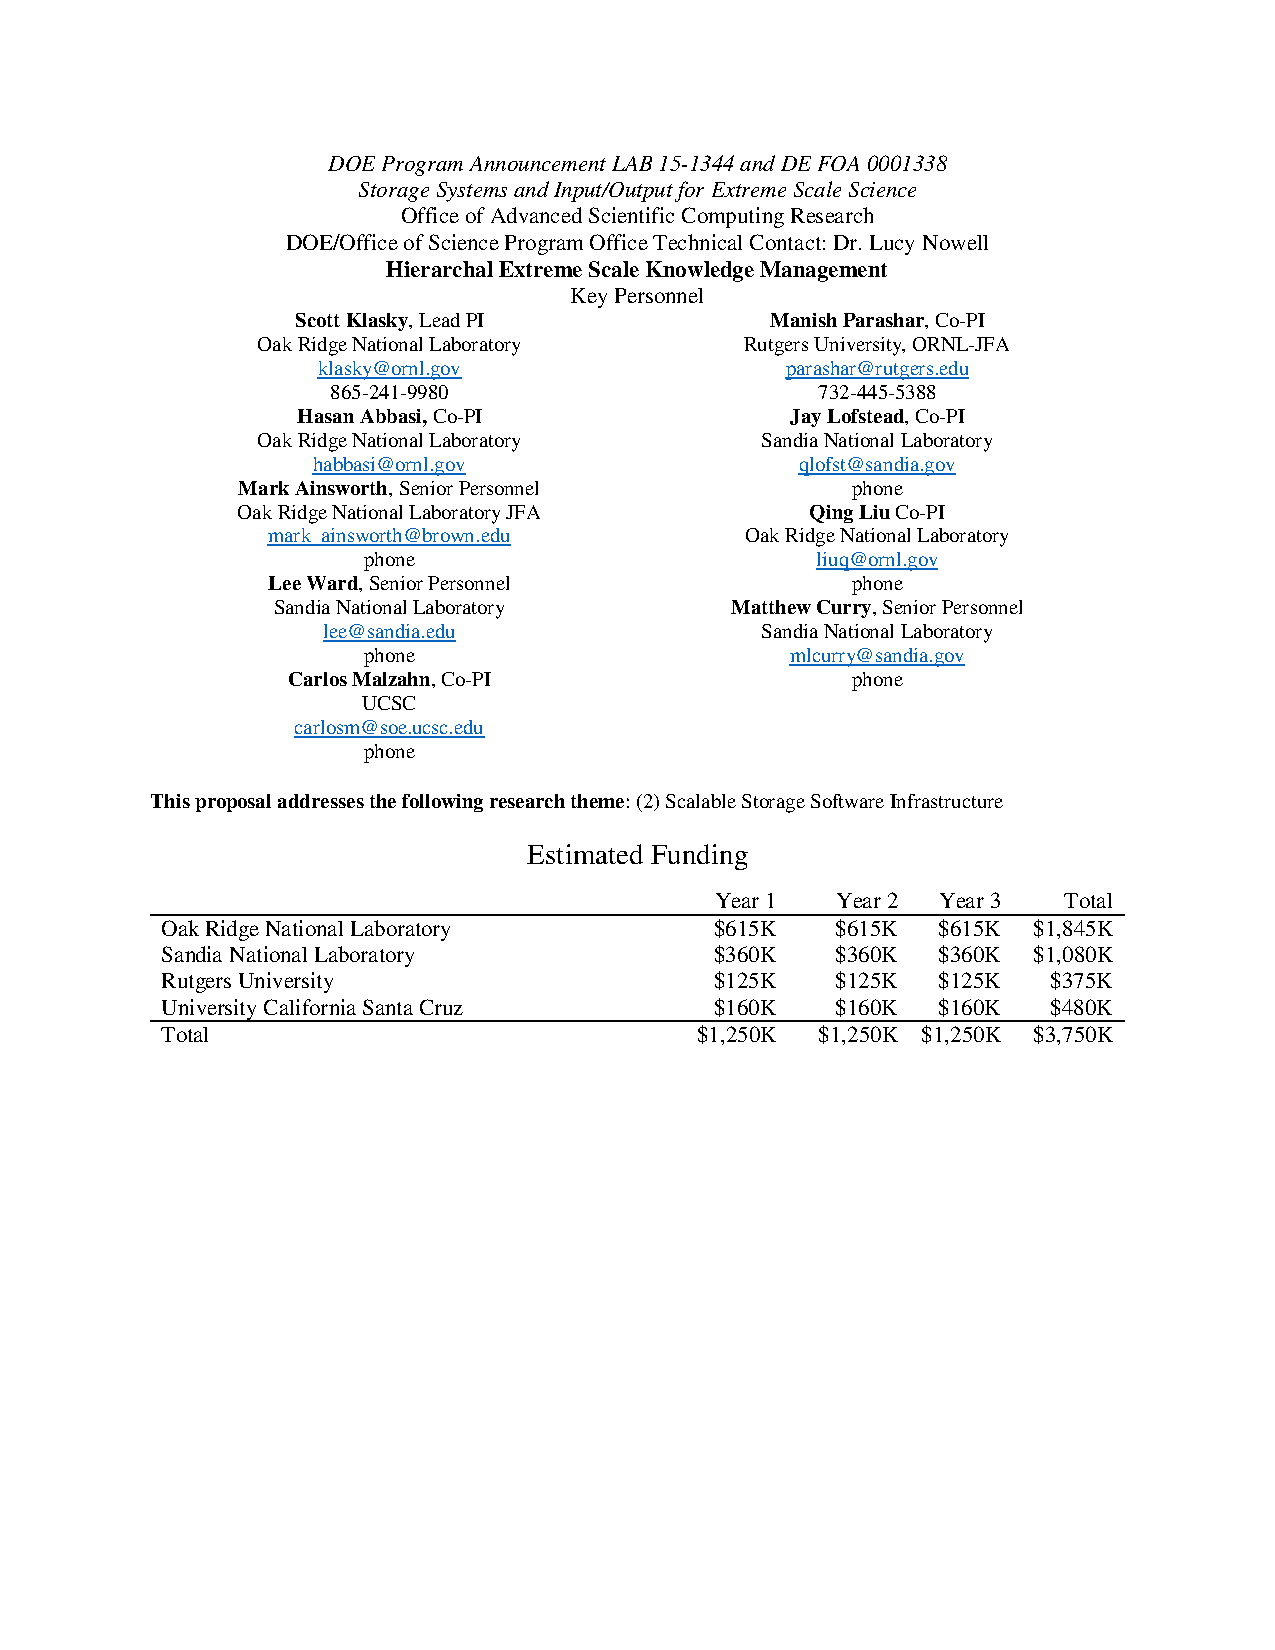
\includepdf[pages={1}]{ornl-cover.pdf}
%\pagebreak

\author{
  \IEEEauthorblockN {
    PI: Scott Klasky, % \IEEEauthorrefmark{1},
    Co-PI Manish Parashar % \IEEEauthorrefmark{1}
  }
  \IEEEauthorblockA {
    % \IEEEauthorrefmark{1}
    Mathematics and Computer Science Division,
    Argonne National Laboratory,
    Argonne, IL, USA}
}

%\maketitle

% Heilmeyer Points: from http://www.csee.umbc.edu/~finin/home/heilmeyerCatechism.html
% 
% \begin{enumerate}

% \item What is the problem, why is it hard? 

% \item How is it solved today?
%  Fig A: much 

% \item What is the new technical idea; why can we succeed now?
%  Integration of proven components into an architecture that solves
%  problems. New research will resolve remaining technical hurdles.

% \item What is the impact if successful?
%  Users and developers will be able to ...

% \item How will the program be organized?
%  Participants and focus areas

% \item How will intermediate results be generated?
%  Toolkit snapshots and application

% \item How will you measure progress?
%  Provide metrics

% \item What will it cost?
%  Cover sheet

% \end{enumerate}
%

{\bf Title of Pre-application:} Hierarchal Extreme Scale Knowledge Management \par
{\bf Principal Investigator:} Scott Klasky, Group Leader, ORNL, 854-241-9980, klasky@ornl.gov \par
{\bf Funding Opportunity Announcement Number: DE-FOA-0001338} \par
{\bf List of all co-PIs and Key/Senior Personnel} \par
Hasan Abbasi, Oak Ridge National Laboratory \par
Mark Ainsworth, Oak Ridge National Laboratory JFA, Brown University \par
Matthew Curry, Sandia National Laboratory\par
Qing Gary Liu, Oak Ridge National Laboratory \par
Jay Lofstead, Sandia National Laboratory \par
Kimmy Mu, Oak Ridge National Laboratory \par
Carlos Malzahn, U. Cal. Santa Cruz \par
Manish Parashar, Rutgers University, Oak Ridge National Laboratory \par
Sudharshan Vazhkudai, Oak Ridge National Laboratory \par
Lee Ward, Sandia National Laboratory \par
\vskip 0.2 in



\underline{\textbf{Objectives:}} Exascale scientific discovery will
%introduce more complex hardware, and many simulations will 
be severely bottlenecked without sufficient new 
 research into managing and storing the large amounts of 
data that will be produced during the simulation, and analyzed for months afterwards.
%Our goal in this project is to investigate a unique approach to addressing this data management 
%and storage challenge for multi-tier exascale storage architectures, thereby expediting insights into mission critical
%scientific processes. 
Our goal in this project is to address the associated I/O and storage challenges on the 
future storage landscape, and expedite insights into mission critical
scientific processes. To this end, we plan
 to research and develop a unique application-aware data management scheme that
can (1) effectively map data to multi-tier exascale storage architectures, 
(2) facilitate how data can be efficiently written to and 
 read from a complex heterogeneous storage hierarchy, and (3) reduce and re-generate
data on-the-fly without compromising the quality of science. The project
will assemble a team with strong expertise in I/O middleware (ORNL, Rutgers), file system (SNL, UCSC)
and storage (UCSC), and connect and coordinate
these key storage components in a seamless fashion. 
% the multi-tier challenges that are faced by scientists in creating and
% managing and storing their data  to expedite insights xsinto
% mission critical scientific processes in exascale compuxsting.
%
%Specifically, we propose a research program that aims to explore a hierarchical
%organization and storage infrastructure that will facilitate how data can
%be written to and read from a complex heterogenous storage hierarchy
%efficiently.  
%
Our approach is to explicitly and implicitly capture user/application intentions 
and use this information, along with direct feedback from the I/O and storage
system, to dynamically structure, organize, process and map the data so that 
it can most effectively support complex I/O patterns. This will be done
with an awareness of data usage semantics and an understanding 
of current and future hardware and software technologies. 
%re-organize and possibly reduce the total amount of information 
%Since data analysis and visualization will be performed in both an
%in situ and post processing environment, we will continue to use our I/O and
%storage abstractions to help enable applications to take full advantage of
%the hardware and software environments. 
On the other hand, data reduction is becoming increasingly important, as a result of 
the disparirty between data volume/frequency and storage bandwdith. 
Rather than focusing solely on lossless 
compression, we will incorporate lossy compression with the ability to annotate 
data, allowing for optimized algorithm selection based on the numerical accuracy
required by the simulation and analysis. We plan to explore this tradeoff of storage 
capacity and bandwidth for computation to determine how to offer the user 
options that can meet their needs with desirable performance characteristics.

%In order to explore the many research challenges in this domain, we will build 
%upon the success of our middleware system, ADIOS, our multi-tier storage 
%system, Sirocco, and our distributed storage system, Ceph.  We will also leverage 
%data staging and data movement technologies, DataSpaces and the Common 
%Communication Interface (CCI), as part of the I/O stack. 
%%used successfully on current leadership class machines. 
%Our experience with this stack will guide us in understanding the new directions for
%research in storage systems and I/O for exascale and beyond systems.

% We will also take advantage of our staging system, Data Spaces, and the
% network abstraction layer, the Common communication Interface (CCI),
% and build on all of
% our sucessful software used in petascale simulations to understand the new directions which need to be understood to fully develop
% the next generation I/O and Storage System for exascale and beyond systems.

%

%
Our objective here is to reduce the time to knowledge, an end-to-end metric
relevant to the scientific discovery process. Beyond the traditional high
volume I/O pattern of checkpoint/restart, we will address the challenges
posed by other essential data access patterns in the knowledge gathering
process. Through a deeper insight into the scientific process we will encode
and utilize accuracy and errors as optimization parameters. 
%
% We will explore access to
% large data sets as part of this process, w

% which means that we will
% also support additional access modes, beyond the traditional
% Checkpoint/Restart methods, and understand that all data has errors
% associated with it and we will ensure that these become encoded to allow for
% additional optimizations. 
For example, scientific simulations contain approximations, as do measurements 
from observations and experiments, and depending on the goal, these approximations 
are acceptable. We can leverage this observation to optimize the presentation of data
to the user and to implement various tradeoffs. For example, users can ask for information 
within a given accuracy bound, allowing us to offer a mode for re-computation vs. data storage
and reterival.

%
{\bf: please list other things from UCSC, OLCF}.
%


\underline{\textbf{Key Technical Approach:}}
%We are fundamentally trying to address the fundmantal questions : 1)  How can we 
%place and mangage massive scienfici data across all of the tiers of the storage and memory
%hiearchy? 2) What are the proper semantics needed in order to help bring knowledge from the applications
%to the middleware layer. 3) What information from the storage layer can be exposed to the middleweare such
%that the placement of information can be agreed upon from what the application requires and what the
%system resources are available. 
Our overall technical approach is based on an application-aware runtime realization of tradeoffs in 
data representation, data placement and data access. We will allow users to ``plug-in'' 
their knowledge about the data, not as bytes but as motifs, allowing the I/O and storage system
to understand user intentions and the relationships between data objects, as well as data
access and transport patterns. This will facilitate
efficient mapping of data from user space, such as a multi-dimensional array, onto various storage tiers. 
Rather than focus on simple data
compression, we will incorporate a multitude of techniques to reduce data on the faster yet smaller
storage tiers, and keep the less
reduced information in the lower storage tiers.

We will support additional data access modes as well. First, within a given
accuracy bounds, offer a mode for re-computation from data stored in a ``fast''
tier to reduce data latencies. Second, exploratory analysis operations
frequently entail an overall data set view followed by targeted data
exploration based on identified features. We will offer support for a
configurable data access mode to support these sorts of analysis accesses. An
``overview'' access mode that gives a quick, approximate within error bounds,
data view that can guide feature selection offering rapid coarse-grained data
exploration without requiring loading the complete, detailed data set from
storage. Based on the granularity requested, the accuracy and size of the data
returned can be adjusted. At the most extreme setting, the original data can
be retrieved at the time cost of moving the potentially huge data quantity.

Third, to ensure available storage for subsequent operations, we will offer
automatic data migration based on user annotations for required data lifetimes
using monitoring and learning techniques. Unlike existing approaches, this will
be tempered both by the user annotations and through learned access patterns.
While past access patterns may not indicate future access because the
simulation run purpose may have changed, we are focused on scalability where
runs are subsequently larger as the simulation prepares for a capability run.
By learning from the output and access patterns during this run sequence, we
can accurate decide how to place and organize data for the critical capability
runs. Fourth, we anticipate storing multiple data copies, each compressed in
different ways according to the underlying media, some of these copies will
disappear based on storage pressures, but data persistence will be maintained
according to user specifications. Assuming a relatively low latency cache layer
before a tape system, we can offer exploratory data access reserving pulling
data from tape to just the data required. This will save scientists time and
make data stored on tape usable without long delays.

Our research efforts will be heavily focused on the need to, in a coordinated
manner, adapt data and metadata retention policies to the dynamic
resource balancing that will need to take place between the application,
OS/R, and hardware.

The success of this project will  provide insights into how to build autonomic middleware and storage layers which can interact
well with each other, and take user-provided hints. Today, data is reduced by application scientist who have 
limited information on what the storage layer can provide. They often make compromises based on this limited knowledge
and either tune their output for writing or reading performance. This data then gets moved to other locations, and much of
the tuning is lost when the data is read back during their post processing. Furthermore, there is a limited set of operations
which users will be able to stage to other staging nodes for real-time-reduction and visualization. 

%We will identify,  through concrete application evaluation, the requirements for highly usable and scalable middleware and storage layers




%\includepdf[pages={1}]{COI.pdf}



\end{document}

%%% End: 
